
\subsection{Variabler Teil}
Während in Normalfall die Anomalie als konstante Beschleunigung angesehen wird, wiesen betreits Anderson et al. in
ihrer Arbeit im Jahr 2002 darauf hin, dass es periodische Anteile von etwa 10\% in der Pioneer-Anomalie zu
geben scheint.
Im Jahr 2008 zeigte die GAP\cite{Levy2008}, dass sich die Qualität des Fits nennenswert steigern lässt, wenn man zusätzlich zur konstanten Beschleunigung periodische Terme verwendet.
Dabei ist es ihnen gelungen, eine Beziehung zwischen dem Unterschied der Azimutalwinkel zwischen Sonde und Erde sowie
den zeitlich veränderlichen Anteilen der Pioneer-Anomalie zu finden. 

\begin{figure}[htnb]
\begin{center}
\noindent    
\psfig{figure=images/variabel,width=\linewidth,height=\textheight,keepaspectratio}
\end{center}
\vskip -10pt
  \caption{Hier sieht man, wie gut die empirisch gefundene Funktion zu den Messwerten passt. G steht für die Antennen in Goldstone, C für Canberra und M für Madrid. Die Funktion wurde nur an die Werte gefittet, bei welchen Sende- und Empfangsantennen in Madrid standen, da diese genauer sind. Man erkennt dabei deutlich die täglichen Variationen.\cite{Levy2009}}\label{fig:variabel}
\end{figure} 

\begin{figure}[htnb]
\begin{minipage}[t]{\linewidth}
	\centering
	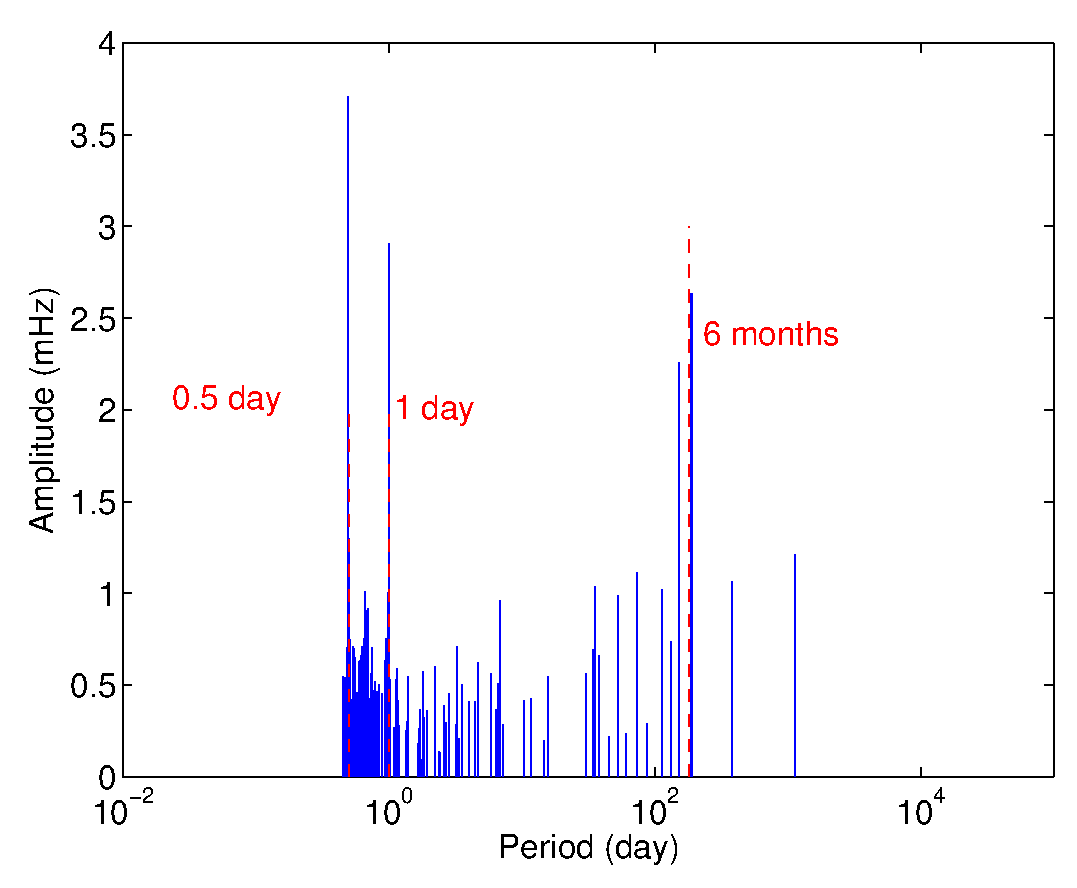
\includegraphics[width=.8\linewidth]{images/SparSpec_begining}
  \caption{SparSpec Analyse der Abweichungen nach einem Fit mit konstanter Anomalie, ohne variable Terme.\cite{Levy2009}}\label{fig:SparSpec_pre}
\end{minipage}
\hfill
\begin{minipage}[t]{\linewidth}
	\centering
	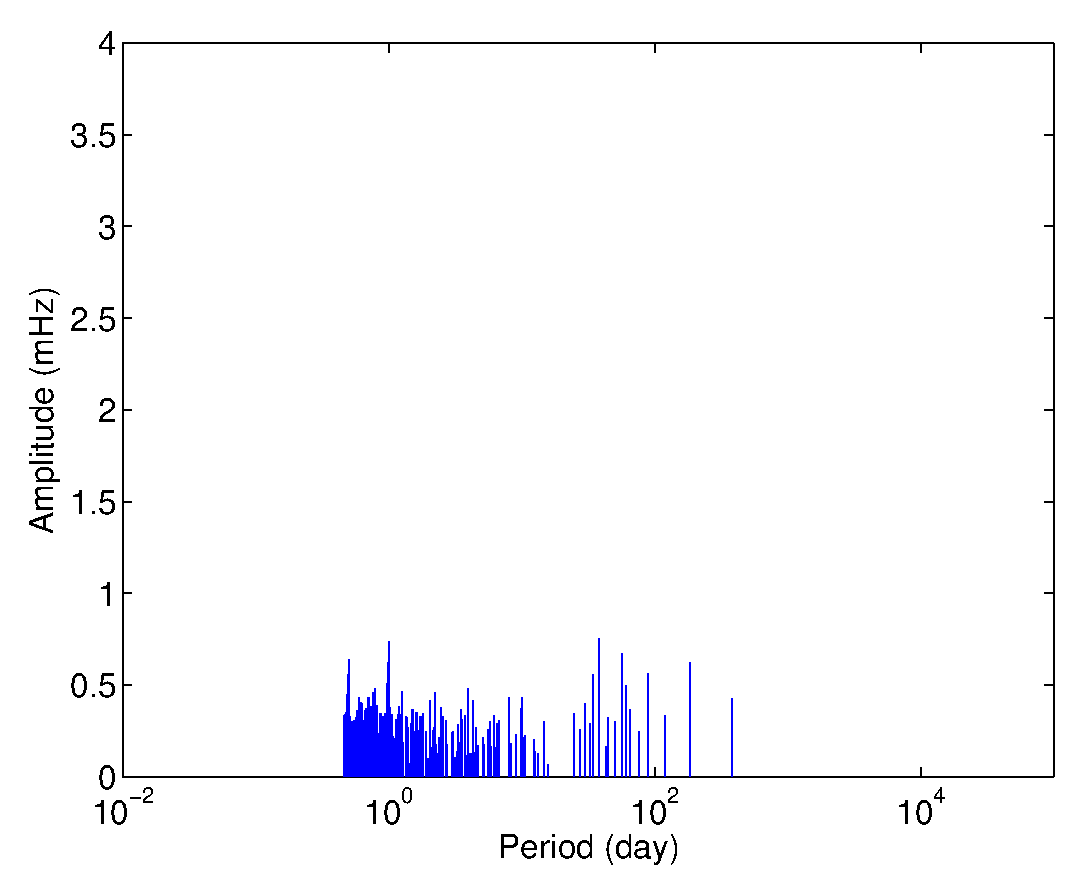
\includegraphics[width=.8\linewidth]{images/SparSpec_end}
  \caption{SparSpec Analyse der Abweichungen nach einem Fit mit konstanter Anomalie und mit variablen Termen.\cite{Levy2009}}\label{fig:SparSpec_post}
\end{minipage}
 \end{figure}

Um die Existenz von periodischen Signalanteilen zu verdeutlichen, tragen die Abweichungen der Messwerte nach Entfernen der konstanten Anomalie im Frequenzbereich auf. Gewöhnlicherweise verwendet man dafür eine Fouriertransformation, da die Messpunkte im Falle der Pioneer-Daten allerdings nicht gleichmäßig verteilt sind, ist dies hier nicht möglich. Statt dessen verwendet man eine Software namens SparSpec.
Die periodischen Anteile des Signals lassen sich auf der daraus erhaltenen Abbildung \ref{fig:SparSpec_pre} sehr gut als herausragende Spitzen erkennen.
Die drei großen Peaks liegen bei $f_1=0.9974\pm0.004\ Tagen$, $f_2=\frac12(0.9972\pm0.004)\ Tagen$ und 
$f_3=189\pm32\ Tagen$, wobei $ 1\ Tag = 60 \cdot 60 \cdot 24 \:s = 86400\:s$ ist.
Bedenkt man das 1.0 siderischer Tag = 0.9972 Tage ist, so entspricht dies genau halbtägigen, täglichen und halbjährlichen Schwankungen.

Die Ursache für diese periodischen Terme dürfte nach gängiger Ansicht nicht in den Sonden zu suchen sein. Fehler im atmosphärischen Modell wären eine naheliegende Ursache für tägliche Variationen. Da diese jedoch von den Konditionen bei den Einrichtungen des DSN abhängen, müssten sie mit der Periode des Sonnentags und nicht des siderischen Tages verlaufen\cite{Levy2009}.
Anderson et al. ziehen für die Variationen Modellierungsfehler – wie Fehler in den Ephemeriden oder der Ausrichtung der Drehachse der Erde, oder fehlerhafte beziehungsweiße zu ungenaue Koordinaten der Messstationen – in Betracht\cite{Levy2009}\cite{Dittus2006}. % originalquelle?
Die Gruppe um Levey (GAP) hält dies jedoch für unwahrscheinlich, da diese Daten durch andere Beobachtungsmethoden
stark gestützt werden und es somit schwer wäre sie stark genug zu verändern um die gemessenen Effekte zu erklären. %Markward: Position offen geht auch

Sie nehmen in ihrer Untersuchung an, dass durch eine beliebige Ursache die Ausbreitung des Tracking-Signals auf
dem Weg zwischen Raumsonde und Erde verändert wird. Sie beschreiben die Ursache als Funktion des Winkels $\varphi$. Dieser wird definiert als die Differenz zwischen dem Azimutalwinkel der Antenne des DSN $\varphi_A$ und dem Azimutalwinkel der Pioneer-Sonde $\varphi_P$: $\varphi=\varphi_A-\varphi_P$. % siehe Grafik
Dieses Modell berücksichtigt also sowohl die Bewegung der Erde um die Sonne, als auch die Rotation der Erde um ihre Achse.
Die Beeinflussung des Signals wird nun mit Fourierkoeffizienten ($\upsilon_n$ und $\upsilon'_n$), beschrieben:
\begin{equation}
\Delta f = \sum_n (\upsilon_n(cos(n\varphi_u)+cos(n\varphi_d))+\upsilon'_n(sin(n\varphi_u)+sin(n\varphi_d))
\end{equation}
wobei $\varphi_u$ und $\varphi_d$ die Winkel $\varphi$ bei Up- beziehungsweise Downlink sind.
Nun können wir die die Fourierkoeffizienten sowie die konstante Anomalie an die Messwerte fitten. Wir verwenden dabei n = 1 und 2, das Hinzufügen von höheren Ordnungen bringt keine nennenswerte Verbesserung.

Dieses geometrische Modell beschreibt sowohl die täglichen als auch die jährlichen
Schwankungen und verringert die Standardabweichung der Messwerte von 9.8 mHz auf 5.5 mHz.
Auch die Spektralanalyse (Abb. \ref{fig:SparSpec_post}) dieses Fits zeigt die Verbesserung deutlich\cite{Levy2008}. % Besser zitieren
%mehr, weiter, ...

% Wie hängt das folgende mit dem obigen zusammen:
Nieto und Anderson weisen in \cite{Nieto2005} des weiteren darauf hin, das sich die jährliche zeitliche Änderung der Anomalie %von wann
grob durch eine Sinuswelle beschreiben lässt. Im Falle von Pioneer 10 hat diese eine Amplitude von $(0.525\pm0.155)\cdot10^{-8}cm/s^{2}$ und im Fall von Pioneer 11 $(0.498\pm0.176)\cdot10^{-8}cm/s^{2}$. Der Phasenunterschied der beiden Wellen beträgt 173.2°, was in etwa dem Winkelunterschied zwischen den ekliptikalen Längen\footnote{Ekliptikale Länge/Breite sind die zwei Himmelskoordinaten des ekliptikalen Koordinatensystems, welche die Ekliptik als Referenz zur Angabe der Position eines Objekts am Himmel verwendet.} der Flugrichtungen der Raumsonden entspricht, während die Amplituden etwa proportional zum Cosinus der ekliptikalen Breiten sind.

%Wohin damit:
Für die Betrachtung der veränderlichen Anteile der Anomalie muss die Kompressionszeit der Daten natürlich immer entsprechend kurz sein\cite{Nieto2005}.

\FloatBarrier